\documentclass[12pt]{article}% use option titlepage to get the title on a page of its own.
\usepackage{pdfpages}
\usepackage{amsmath}
\usepackage{blindtext}
\usepackage{amssymb}
\usepackage{graphicx}
\usepackage{listings}
\usepackage {tikz}
\usetikzlibrary{shapes.geometric, arrows}
\usetikzlibrary {positioning}

\newcommand\tab[1][1cm]{\hspace*{#1}}
\usepackage{float}

\usepackage[font=small,skip=0pt]{caption}


\begin{document}
\begin{figure}
\begin{center}
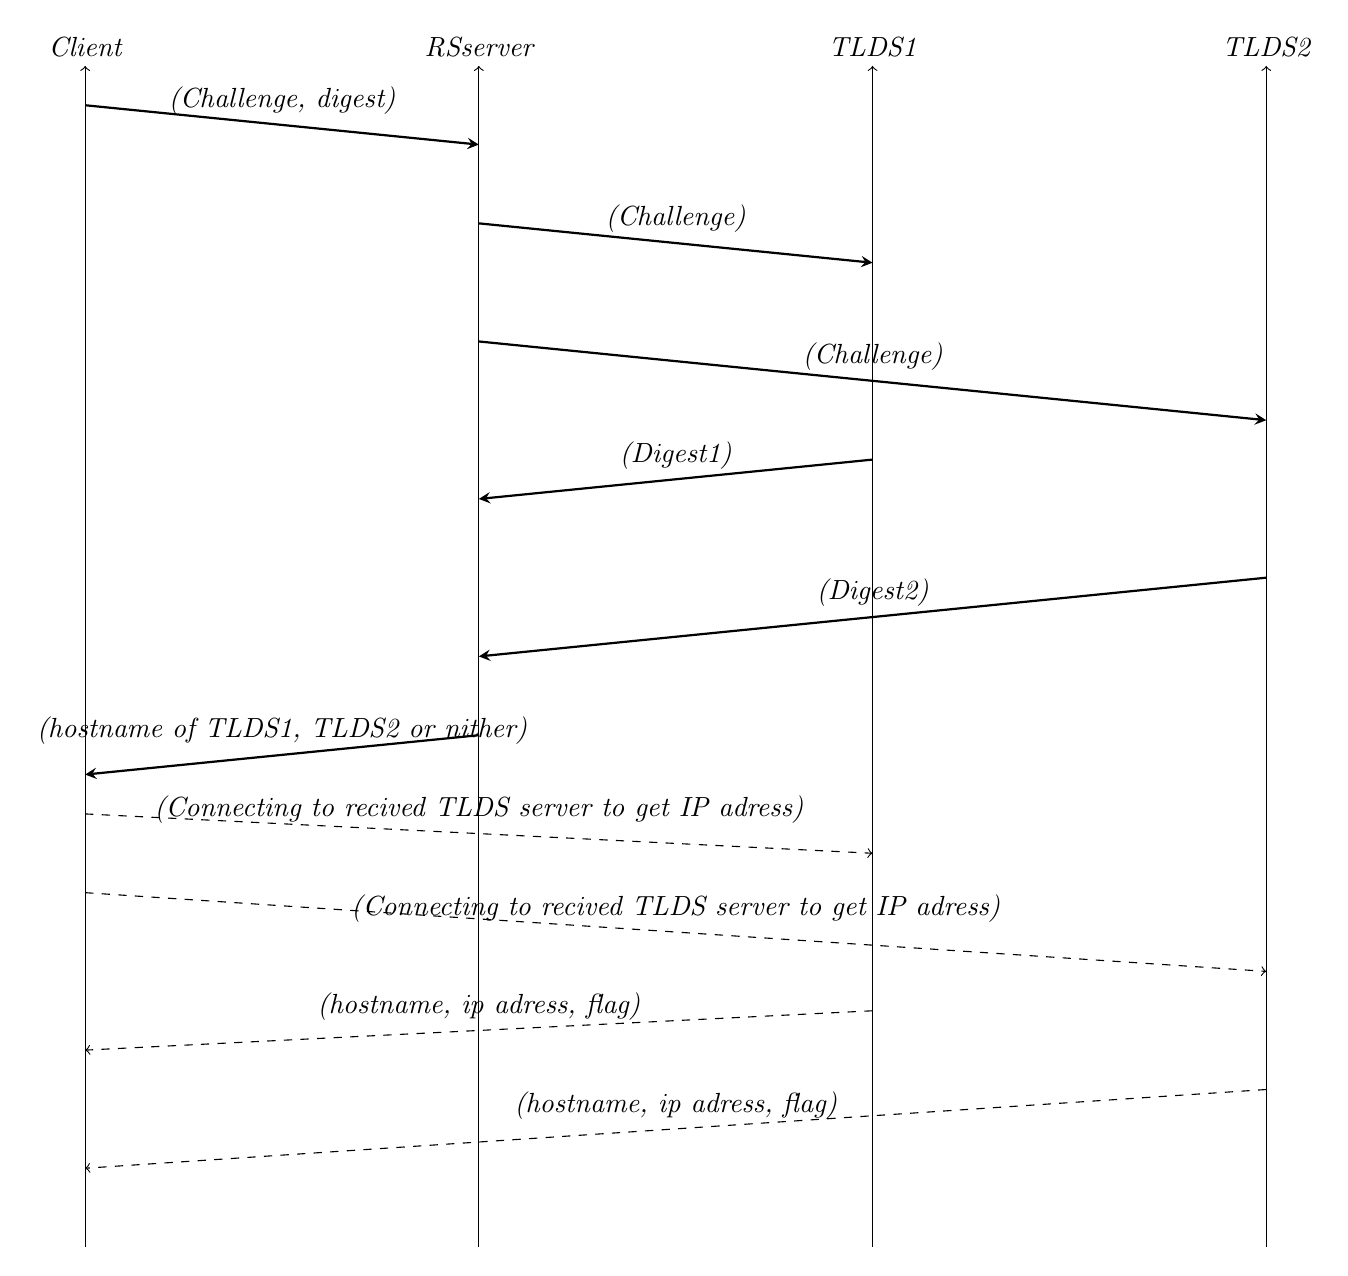
\begin{tikzpicture}
\tikzstyle{arrow} = [thick,->,>=stealth]

%Four vertical linens to represent each server
 \draw[->] (-5,0) -- (-5,15) node [pos=1, above] {\itshape Client};
\draw[->] (0,0) -- (0,15) node [pos=1, above] {\itshape RSserver};
\draw[->] (5,0) -- (5,15) node [pos=1, above] {\itshape TLDS1};
   \draw[->] (10,0) -- (10,15) node [pos=1, above] {\itshape TLDS2};

%Communication from client to RSserver:
 \draw[arrow] (-5,14.5) -- (0,14) node [pos=0.5, above] {\itshape (Challenge, digest)};
 
%Communication from RSserver to both TLDS servers:
 \draw[arrow] (0,13) -- (5,12.5) node [pos=0.5, above] {\itshape (Challenge)};
 \draw[arrow] (0,11.5) -- (10,10.5) node [pos=0.5, above] {\itshape (Challenge)};
 
%Respoce back to RSserver from TLDS servers:
 \draw[arrow] (5,10) -- (0,9.5) node [pos=0.5, above] {\itshape (Digest1)};
 \draw[arrow] (10,8.5) -- (0,7.5) node [pos=0.5, above] {\itshape (Digest2)};

%Connect back to Client with hostname of correct TLDS1 server
 \draw[arrow] (0,6.5) -- (-5,6) node [pos=0.5, above] {\itshape (hostname of TLDS1, TLDS2 or nither)};
 
%Connecting to recived hostname:
 \draw[dashed,->] (-5,5.5) -- (5,5) node [pos=0.5, above] {\itshape (Connecting to recived TLDS server to get IP adress)};
 \draw[dashed,->] (-5,4.5) -- (10,3.5) node [pos=0.5, above] {\itshape (Connecting to recived TLDS server to get IP adress)};

%Getting IP adress desired hostname
 \draw[dashed,->] (5,3) -- (-5,2.5) node [pos=0.5, above] {\itshape (hostname, ip adress, flag)};
\draw[dashed,->] (10,2) -- (-5,1) node [pos=0.5, above] {\itshape (hostname, ip adress, flag)};

\end{tikzpicture}
\end{center}
\end{figure}
\end{document}